\section{Neuronale Netze} %TODO: Absplitten

\subsection{Aufbau und Namenskonventionen}
\begin{figure}[ht!]
  \centering
    \def\layersep{2.5cm}

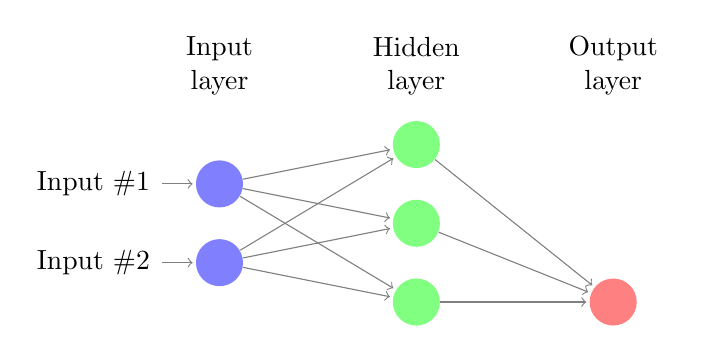
\begin{tikzpicture}[shorten >=1pt,->,draw=black!50, node distance=\layersep]
    \tikzstyle{every pin edge}=[<-,shorten <=1pt]
    \tikzstyle{neuron}=[circle,fill=black!25,minimum size=17pt,inner sep=0pt]
    \tikzstyle{input neuron}=[neuron, fill=blue!50];
    \tikzstyle{output neuron}=[neuron, fill=red!50];
    \tikzstyle{hidden neuron}=[neuron, fill=green!50];
    \tikzstyle{annot} = [text width=4em, text centered]

    % Draw the input layer nodes
    \foreach \name / \y in {1,...,2}
    % This is the same as writing \foreach \name / \y in {1/1,2/2,3/3,4/4}
        \node[input neuron, pin=left:Input \#\y] (I-\name) at (0,-\y) {};

    % Draw the hidden layer nodes
    \foreach \name / \y in {1,...,3}
        \path[yshift=0.5cm]
            node[hidden neuron] (H-\name) at (\layersep,-\y cm) {};

    % Draw the output layer node
    %\node[output neuron,pin={[pin edge={->}]right:Output}, right of=H-3] (O) {};
    \node[output neuron, right of=H-3] (O) {};

    % Connect every node in the input layer with every node in the
    % hidden layer.
    \foreach \source in {1,...,2}
        \foreach \dest in {1,...,3}
            \path (I-\source) edge (H-\dest);

    % Connect every node in the hidden layer with the output layer
    \foreach \source in {1,...,3}
        \path (H-\source) edge (O);

    % Annotate the layers
    \node[annot,above of=H-1, node distance=1cm] (hl) {Hidden layer};
    \node[annot,left of=hl] {Input layer};
    \node[annot,right of=hl] {Output layer};   

  %   \node[annot,below of=H-5, node distance=2cm] (hk) {
  %       \[%Matrix Input    
		% \begin{pmatrix}
		% h_{1, 1} \\
		% h_{1, 2} \\
		% h_{1, 3} \\
		% \vdots \\
		% h_{1, m} 
		% \end{pmatrix}\]
  %   };

  %   \node[annot,left of=hk] {
  %   	\[\begin{pmatrix}
		% 1 \\
		% x_{1} \\
		% x_{2} \\
		% \vdots \\
		% x_{m} 
		% \end{pmatrix}\]
  %   };
  %   \node[annot,right of=hk] {
  %   	\[\begin{pmatrix}
		% y_{1} \\
		% y_{2} \\
		% \vdots \\
		% y_{m} 
		% \end{pmatrix}\]
  %   };

\end{tikzpicture}

  \caption{Ein 2-schichtiges MLP.}
  \label{fig:MLP}
\end{figure}


Ein Neuronales Netz (zur Abgrenzungen zu biologischen Netzen in der Fachliteratur als Artificial Neural Network (ANN) bezeichnet) besteht aus mehreren Schichten Neuronen: einem Input Layer, einem (oder mehreren) Hidden Layer, und einem Output Layer. 
Wenn man von einem k-schichtigen ANN spricht, bezeichnet k die Anzahl der Schichten, ohne Input-Layer.

Die Ausgabe der Eingabeneuronen entspricht den jeweiligen Elementen des Eingabevektors.
Die Hidden-Layer besten aus Neuronen mit einer nicht linearen Aktivierungsfunktion, die die Eingangsdaten transformiert.

Jeder Layer ist mit den anderen elementweise verbunden. Jede Verbindung hat ein so genanntes Gewicht $w_{ij} \in \mathbb{R}$. Daten fließen nur von links nach rechts. Netzwerke dieser Art heißen Multilayer-Perceptrons (MLP). 

In Abbildung \ref{fig:MLP} sieht man ein typisches MLP. In dieser Abbildung fehlt aber noch ein wichtiges, spezielles Neuron mit den dazu gehörigen Gewichten: der Bias. Er dient dazu, die Eingabewerte jedes Neurons noch um einen linearen Wert zu ergänzen. Dadurch wird das Training erleichtert und die Mächtigkeit des Modells wird gestärkt. In der Praxis wird er wie ein spezielles Neuron mit konstanter Aktivierung $+1$ behandelt, das eine Verbindung (inklusive Gewicht) zu jedem Neuron, das nicht im Input Layer ist, besitzt. Es wird dann als nulltes Neuron jeder Schicht im Gewichtsvektor angesehen - das erleichtert uns dann Berechnungen.
 

\subsection{Die Aktivierungsfunktion}

Die Funktion, die pro Knoten die nicht-lineare Transformation durchführt, heißt Aktivierungsfunktion. 

Häufig wird eine Funktion mit sigmoiden Erscheinungsbild gewählt, das heißt eine Funktion, die die Ergebnisse in ein bestimmtes Intervall komprimiert und ein an ein S erinnerndes Erscheinungsbild hat. 

Beispiele für Funktion diesen Typs sind die so genannte logistische Funktion

\begin{equation}
\sigma_1(x) = \frac{1}{1+e^{-x}}.
\end{equation}

und der hyperbolische Tangens

\begin{equation}
\sigma_2(x) = \tanh(x) = \frac{1-e^{-2x}}{1+e^{-2x}} = 
\sigma_1(2x) -1.
\end{equation}

Er hat aber einen Nachteil mit der logistischen Funktion gemeinsam: sehr kleine oder sehr große Werte haben eine sehr kleine Ableitung zur Folge. Da die Ableitung der Aktivierungsfunktion beim Training (vgl.~Formel \ref{eq:backpropagation}) benutzt wird, kann das ein Absterben des Neurons zur Folge haben. 

In \cite{lecunefficient} wird $1.7159 \tanh(\frac{2}{3} x)$ empfohlen, wenn eine Normalisierung vorgenommen wird. 

Eine alternative Aktivierungsfunktion ist die Rectifier-Funktion 

\begin{equation}
\sigma_3(x) = \max(0,x).
\end{equation} 

In \cite{glorot2011deep} wird argumentiert, dass die logistische Funktion zwar biologisch plausibler ist als der hyperbolische Tangens, aber die Rectifier Funktion noch näher an der Funktionsweise biologischer Neuronen ist. Was für uns relevanter ist: sie ist effizienter zu berechnen. Sie ist also in der Praxis oft eine bessere Wahl. 

Problematisch ist bei der Rectifier-Funktion jedoch, dass durch $x < 0$ das Neuron abstirbt, weil die Ableitung gleich 0 ist: Beim Training des Modells kann ein Fehler nicht korrigiert werden. Für $x = 0$ ist die Funktion gar nicht ableitbar, für beliebig nahe Werte jedoch schon\cite{bengio2012practical}. 

\subsection{Die Kostenfunktion}
Wir benutzen eine Kostenfunktion, die den Fehler des Netzes quantifiziert.

Die Maximum-Likelihood-Methode wird benutzt, um, wenn Beobachtungen gegeben sind, die Parameter einer Wahrscheinlichkeitsverteilung zu schätzen. Dazu betrachten wir Neuronale Netze als Modell für eine Wahrscheinlichkeitsverteilung.

Wir nehmen jetzt an, dass die Beobachtungen $x_1, \ldots , x_n$ unabhängig und identisch verteilt sind. Dann sieht die Funktion für die Parameter $\theta$ folgendermaßen aus:

\begin{equation}
  \mathcal{L} (\theta; x_1, \ldots, x_n) =
  f(x_1, x_2, \ldots, x_n | \theta) =
  \prod_{i = 1}^n f(x_i|\theta) .
\end{equation}

Sie beschreibt die Likelihood, das ist die Funktion eines Parameters, für ein gegebenes Resultat. Interessant ist, dass wir bei dieser Funktion die Beobachtungen als feste Parameter der Funktion ansehen, die eigentlichen Parameter sind dann variabel. Wir optimieren also die Wahrscheinlichkeitsverteilungsfunktion. Dafür wird die Likelihood-Funktion $\mathcal{L}$ maximiert.

Anstatt die Maximum-Likelihood-Funktion zu maximieren, minimieren wir die negative, logarithmische Maximum-Likelihood-Funktion. Das funktioniert, weil der Logarithmus eine monotone Funktion ist, es erleichtert uns außerdem, mit großen Werten zu rechnen. Die resultierende Funktion sieht folgendermaßen aus:
\begin{align}
 E  & = - \ln \mathcal{L} \\
  %& = -  \ln \left( \prod_{i = 1}^n f(x_i|\theta) \right) \\
  & = - \sum_{i=1}^n \ln f(x_i|\theta).
\end{align}

Aus dieser allgemeinen Fehlerfunktion lassen sich spezielle Fehlerfunktionen ableiten, die in der Praxis benutzt werden\cite{bishop1995neural}:

Wir wollen jetzt wieder den Fehler für $p(t|\theta)$ darstellen. Wir nehmen an, dass die Variable $t_k$ aus einer deterministischen Funktion und normal-verteiltem Rauschen (mit Erwartungswert $0$ und Varianz $\sigma$) gebildet wird.  
Deswegen gilt: %Umformulieren? p(t|k)? Was bedeutet das?
\begin{equation}
  p(t_k|\theta) = \frac{1}{(2 \pi \sigma^2)^{0.5}} \exp \left( -\frac{ \left[  y_k - t_k \right]^2 }{2 \sigma^2} \right).
\end{equation}.

Den Fehlerterm können wir jetzt einfach als Summe über alle Fehlerwahrscheinlichkeiten darstellen:
\begin{equation}
  E = \frac{1}{2 \sigma^2} \sum_{n=1}^{N} \sum_{k=1}^{c} \left[ y_k - t_k^n \right]^2 + Nc \ln \sigma + \frac{N_c}{2} \ln (2 \pi).
\end{equation}

Ignorieren wir nun alle Faktoren, die nicht von den Parametern des Netzes abhängen, erhalten wir 
\begin{equation}
\label{eq:MSE}
E = \frac{1}{2} \sum_{n=1}^N \sum_{k=1}^c \left( y_k^n - t_k^n \right)^2,
\end{equation}

wobei $y^k$ dem Ausgabevektor des Netzwerks für den Fall $k$ und $t^k$ der gewollten Ausgabe entspricht.
Diese Fehlerfunktion heißt Mean-square-error (MSE)\cite{bishop1995neural}.

Eine für Klassifizierungsprobleme oft benutze Fehlerfunktion ist die negative Kreuzentropie:
\begin{equation}
\label{eq:crossEntropy}
    E = -\sum_{n} \sum_{k=1}^c t_k^n \ln y_k^n ,
\end{equation}

wobei $t_k^n \in (0,1)$ der Wahrscheinlichkeit, dass die Eingabe $x^n$ in der Klasse $c$ ist, entspricht. 

Sie ist für diese Problemklasse stochastisch schöner zu interpretieren und wird normalerweise mit der Softmax-Aktivierungsfunktion (\ref{eq:softmax}) benutzt\cite{bishop1995neural}.

\subsection{Feedforward}
Um ein ANN zur Vorhersage neuer Input-Vektoren zu benutzen, wird es im sogenannten Feedforward Modus betrieben. In diesem wird der Input Vektor zuerst den Neuronen des Input-Layers präsentiert. Alle anderen Neuronen des nächsten Layers bilden dann eine lineare Kombination aus den Neuronen ihrer Vorgängerschicht: 
\begin{equation}
\label{eq:feedforward1}
\text{net}_j = \sum_{i} w_{ji} y_i = w_j^t y.
\end{equation}

Bei dieser Formel ist $w_{ji}$ das Gewicht vom Neuron $j$ zum Neuron $i$. Die Summe lässt sich auch auch als Skalarprodukt $w_j^t y$ darstellen, wobei die Spalten von $w$ den Gewichten der Layers entsprechen. %TODO: Formulierung!

Nachdem diese lineare Transformation abgeschlossen ist, wird bei allen Neuronen (außer bei denen im Output-Layer) die Aktivierungsfunktion benutzt, die dann eine nicht-lineare Transformation durchführt: 
\begin{equation}
\label{eq:feedforward2}
y_j = \sigma (\text{net}_j).
\end{equation}

Dieser Prozess wird so lange durchgeführt, bis die Daten das komplette Netz durchlaufen haben, und im Output-Layer ankommen\cite{bishop1995neural}.


\subsection{Die Minimierung der Kostenfunktion - Backpropagation}

Natürlich reicht es für maschinelles Lernen nicht aus, nur Vorhersagen zu treffen - das Modell muss sich auch anpassen können. Bei Neuronalen Netzen heißt der benutzte Trainingsalgorithmus Backpropagation.

Es ist eine Möglichkeit den Fehler, der bei den Ausgabeneuronen auftritt, auch für die Neuronen der Schichten davor zu berücksichtigen - der Fehler wird zurückgesendet.

Dazu wird als erster Schritt für einen Trainingsvektor ein Forward-Pass durchgeführt - damit wird die Vorhersage des Netzwerkes berechnet, und anschließend mit der vorgegeben Lösung des Trainingssets verglichen.

Diese Werte werden dann benutzt, um den Fehler zu berechnen, und dann die Parameter (also die Gewichte) anzupassen.

Am Ende wird das Ergebnis der Optimierungsmethode benutzt, um die Gewichte zu aktualisieren. Dieser Algorithmus wurde zuerst in \cite{rumelhart1988learning} erfunden, wir benutzen aber eine etwas modernere Formulierung inspiriert von \cite{bishop1995neural, duda2012pattern}. 

Alle relevanten Fehlerfunktionen haben die Form 
\begin{equation}
E = \sum_n E_n(y_1, \ldots, y_c),
\end{equation}

das heißt, der Gesamtfehler ist die Summe aller Einzelfehler.
Wir nehmen weiterhin an, dass der Fehler als ableitbare Funktion der Ausgabe-Werte darstellbar ist.
Für die folgende Herleitung benutzen wir die MSE-Kostenfunktion (\ref{eq:MSE}), für andere Fehlerfunktionen ist die Vorgehensweise analog.

Wir suchen jetzt die partielle Ableitung der Fehlerfunktion unter Berücksichtigung eines bestimmten Gewichts:
\begin{equation}
\frac{\partial E^n}{\partial w_{i,j}} = \frac{\partial E^n}{\partial net_j}  \frac{\partial net_j }{\partial w_{ji}}.
\end{equation}

Wir definieren jetzt die Hilfsvariablen:
\begin{IEEEeqnarray}{rCl}
\frac{\partial net_j }{\partial w_{ji}} & = & y_i \quad \text{und}
\\
\frac{\partial E^n}{\partial net_j} & = & \delta_j,
\end{IEEEeqnarray}

wobei $y_i$ durch den Feedforward-Pass (also mit den Formeln \ref{eq:feedforward1} und \ref{eq:feedforward2}) berechnet wird. 

Mit diesen Variablen können wir die Ableitung schön beschreiben als
\begin{equation}
\label{eq:evaluate}
  \frac{\partial E^n}{\partial w_{ij}} = y_i \delta_j.
\end{equation}

Durch mehrfaches Anwenden der Kettenregel bekommen wir die so genannte Backpropagation-Formel:
\begin{equation}
\label{eq:backpropagation}
\delta_j =  \begin{cases}
               \sigma ' (net_j) (y_j - t_j)          & \text{wenn j $\in$ Ausgabeschicht}\\
               \sigma ' (net_j) \sum_k w_{kj} \delta_k     & \text{wenn j $\in$ Hiddenlayer}.
           \end{cases} 
\end{equation} 

Um den Gradienten zu berechnen müssen wir nun nur noch $\delta_j$ rekursiv bei den Ausgabeneuronen beginnend mit \ref{eq:backpropagation} berechnen, und dann mit \ref{eq:evaluate} auswerten \cite{bishop1995neural}. 

Wichtig ist noch die Unterscheidung zwischen:

\begin{LaTeXdescription}
	\item[Stochastic Backpropagation]
	Bei diesem Verfahren wird immer nur ein zufällig ausgewählter Eingabevektor pro Iteration evaluiert, dann werden sofort die Gewichte aktualisiert. Wenn er zusammen mit dem Gradientenverfahren benutzt wird, sprechen wir von Stochastic Gradient Descent (SGD).
	\item[Batch Backpropagation] 
	Bei der zweiten Methode werden alle Eingabevektoren des Trainingssets präsentiert und die Gewichtsänderungen summiert. Erst dann werden alle Gewichte aktualisiert.\cite{duda2012pattern}
\end{LaTeXdescription}

Die stochastische Methode ist die in der Praxis bevorzugte, weil die Konvergenz nicht von der Größe des Trainingssets, sondern viel mehr von der Anzahl der Iterationen und der Verteilung der Trainingsdaten abhängt - für große Sets ist ein Benutzen der Batch Methode nicht mehr sinnvoll \cite{bengio2012practical}.
Ein weiter Vorteil ist, dass sie redundante Trainingsdaten (die bei einem Training für Mustererkennung zwangsläufig auftreten) ausnutzt. Außerdem konvergiert sie eventuell zu einem besseren Minimum als die Batch Methode \cite{lecunefficient}.
Wir werden hier primär die stochastische Methode betrachten, da sie in der Praxis die Bessere ist \cite{lecunefficient, bengio2012practical}.


\subsection{Die numerische Methode - Gradient Descent und verwandte}

Der Gradient wird oft mit dem Gradientenverfahren, einer Methode um Funktionen zu minimieren, benutzt \cite{bishop1995neural,bengio2012practical}.

Das Gradientenverfahren können wir als Iterationsvorschrift darstellen:
\begin{equation}
x_{n+1}=x_n- \eta  \nabla F(x_n), 
\end{equation}

wobei $\nabla$ der Gradient ist, $\nabla_w$ ist der Gradient im Bezug auf die Gewichte. 
Die Konstante $\eta$ heißt Lernrate. Je größer sie ist, desto schneller konvergiert das Verfahren - bei einer zu hoch gewählten sind aber oft Oszillationen oder Stagnation zu beobachten. 

Das Verfahren funktioniert, weil der negative Gradient in die Richtung zeigt, in der die Funktion am schnellsten kleiner wird. Daher kommt auch die Bezeichnung Verfahren des steilsten Abstiegs.

Auf ANNs angewandt, sieht die Formel dann für jeden Zeitschritt $t$ folgendermaßen aus:
\begin{equation}
  \Delta_w^t = - \eta  \nabla_w E(w;t).
\end{equation}
Dabei entspricht $\nabla_w E(w;t)$ dem Gradienten der Fehlerfunktion bezüglich der Gewichte ausgewertet für einen Trainingsvektor $t$.

Das Gradientenverfahren hat das Problem, dass es oft in lokalen Minima stecken bleibt - das ist vor allem bei ANNs problematisch, weil die gewählte Kostenfunktion in den meisten Fällen mehrere lokale Minima besitzt. Auch wenn es nicht unbedingt notwendig, oder sogar erwünscht ist, einen globalen Extremwert zu finden (vgl. \ref{sec:overfitting}), existieren bessere numerische Verfahren. 

Eine Verbesserung zum gewöhnlichen Gradientenverfahren ist es, einen so genannten Momentumparameter zu benutzen, der auch vorherige Ergebnisse einbezieht, und somit das oft beobachtete oszillierende Verhalten des Gradientenverfahrens behebt:
\begin{equation}
 \Delta_w^t = - \eta  \nabla_w J(w) + \gamma \Delta_w^{t-1}.
\end{equation}

Diese Formel ist für $\gamma = 0$ äquivalent zum normalen Gradientenverfahren. Je größer $\gamma$ gewählt wird, desto stärker ist die Auswirkung vergangener Iterationen. 

Bei einigen Problemen kann das Verfahren Vorteile bringen (primär bei Batch Backpropagation \cite{lecunefficient}), oft ist aber SGD mit einer guten Wahl der Lernrate bereits optimal\cite{bengio2012practical}.
